\documentclass[]{article}
\usepackage{lmodern}
\usepackage{amssymb,amsmath}
\usepackage{ifxetex,ifluatex}
\usepackage{fixltx2e} % provides \textsubscript
\ifnum 0\ifxetex 1\fi\ifluatex 1\fi=0 % if pdftex
  \usepackage[T1]{fontenc}
  \usepackage[utf8]{inputenc}
\else % if luatex or xelatex
  \ifxetex
    \usepackage{mathspec}
  \else
    \usepackage{fontspec}
  \fi
  \defaultfontfeatures{Ligatures=TeX,Scale=MatchLowercase}
\fi
% use upquote if available, for straight quotes in verbatim environments
\IfFileExists{upquote.sty}{\usepackage{upquote}}{}
% use microtype if available
\IfFileExists{microtype.sty}{%
\usepackage{microtype}
\UseMicrotypeSet[protrusion]{basicmath} % disable protrusion for tt fonts
}{}
\usepackage[margin=1in]{geometry}
\usepackage{hyperref}
\hypersetup{unicode=true,
            pdftitle={Analysis of Tissue Weights from HFD/Dexamethasone Studies},
            pdfauthor={Innocence Harvey and Dave Bridges},
            pdfborder={0 0 0},
            breaklinks=true}
\urlstyle{same}  % don't use monospace font for urls
\usepackage{longtable,booktabs}
\usepackage{graphicx,grffile}
\makeatletter
\def\maxwidth{\ifdim\Gin@nat@width>\linewidth\linewidth\else\Gin@nat@width\fi}
\def\maxheight{\ifdim\Gin@nat@height>\textheight\textheight\else\Gin@nat@height\fi}
\makeatother
% Scale images if necessary, so that they will not overflow the page
% margins by default, and it is still possible to overwrite the defaults
% using explicit options in \includegraphics[width, height, ...]{}
\setkeys{Gin}{width=\maxwidth,height=\maxheight,keepaspectratio}
\IfFileExists{parskip.sty}{%
\usepackage{parskip}
}{% else
\setlength{\parindent}{0pt}
\setlength{\parskip}{6pt plus 2pt minus 1pt}
}
\setlength{\emergencystretch}{3em}  % prevent overfull lines
\providecommand{\tightlist}{%
  \setlength{\itemsep}{0pt}\setlength{\parskip}{0pt}}
\setcounter{secnumdepth}{0}
% Redefines (sub)paragraphs to behave more like sections
\ifx\paragraph\undefined\else
\let\oldparagraph\paragraph
\renewcommand{\paragraph}[1]{\oldparagraph{#1}\mbox{}}
\fi
\ifx\subparagraph\undefined\else
\let\oldsubparagraph\subparagraph
\renewcommand{\subparagraph}[1]{\oldsubparagraph{#1}\mbox{}}
\fi

%%% Use protect on footnotes to avoid problems with footnotes in titles
\let\rmarkdownfootnote\footnote%
\def\footnote{\protect\rmarkdownfootnote}

%%% Change title format to be more compact
\usepackage{titling}

% Create subtitle command for use in maketitle
\newcommand{\subtitle}[1]{
  \posttitle{
    \begin{center}\large#1\end{center}
    }
}

\setlength{\droptitle}{-2em}
  \title{Analysis of Tissue Weights from HFD/Dexamethasone Studies}
  \pretitle{\vspace{\droptitle}\centering\huge}
  \posttitle{\par}
  \author{Innocence Harvey and Dave Bridges}
  \preauthor{\centering\large\emph}
  \postauthor{\par}
  \predate{\centering\large\emph}
  \postdate{\par}
  \date{April 7, 2017}


\begin{document}
\maketitle

{
\setcounter{tocdepth}{2}
\tableofcontents
}
\section{Data Entry}\label{data-entry}

This script generates figures from the tissue weights found in
../../data/raw/HFD and Chow Tissue Weights.csv. This file is located in
/Users/davebrid/Documents/GitHub/CushingAcromegalyStudy/scripts/scripts-obesity
and was most recently updated on Tue Aug 8 19:28:21 2017.

\section{Number of Animals}\label{number-of-animals}

\begin{longtable}[]{@{}lllr@{}}
\caption{Number of mice in each group}\tabularnewline
\toprule
Status & Diet & Treatment & Number\tabularnewline
\midrule
\endfirsthead
\toprule
Status & Diet & Treatment & Number\tabularnewline
\midrule
\endhead
Fasted & NCD & Water & 8\tabularnewline
Fasted & NCD & Dexamethasone & 8\tabularnewline
Fasted & HFD & Water & 22\tabularnewline
Fasted & HFD & Dexamethasone & 12\tabularnewline
Fed & NCD & Water & 4\tabularnewline
Fed & NCD & Dexamethasone & 4\tabularnewline
\bottomrule
\end{longtable}

\section{Summary Data}\label{summary-data}

The remainder of this analysis is only for Fasted animals

\begin{longtable}[]{@{}llrrrr@{}}
\caption{Averaged Values}\tabularnewline
\toprule
Diet & Treatment & iWAT\_mean.na & eWAT\_mean.na & TS\_mean.na &
Quad\_mean.na\tabularnewline
\midrule
\endfirsthead
\toprule
Diet & Treatment & iWAT\_mean.na & eWAT\_mean.na & TS\_mean.na &
Quad\_mean.na\tabularnewline
\midrule
\endhead
NCD & Water & 141 & 187 & 163 & 240\tabularnewline
NCD & Dexamethasone & 111 & 173 & 144 & 198\tabularnewline
HFD & Water & 841 & 1136 & 191 & 242\tabularnewline
HFD & Dexamethasone & 287 & 464 & 127 & 140\tabularnewline
\bottomrule
\end{longtable}

\section{Muscle Barplots}\label{muscle-barplots}

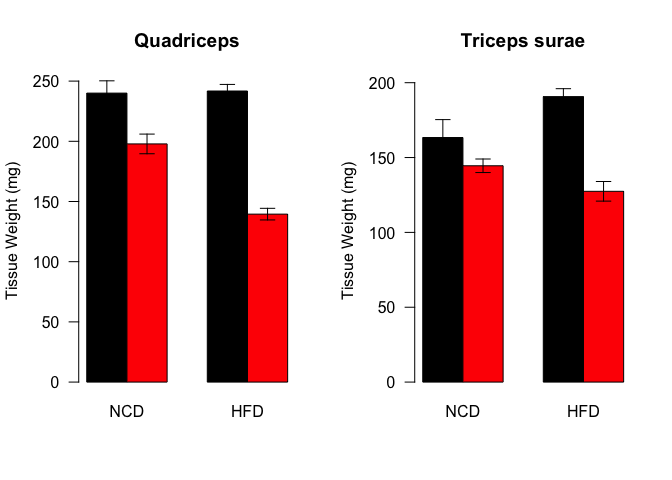
\includegraphics{figures/muscle-weight-barplot-1.png}

\section{Adipose Barplots}\label{adipose-barplots}

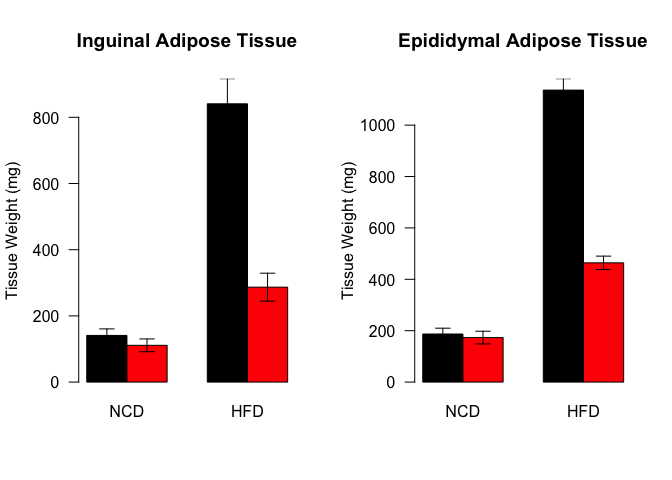
\includegraphics{figures/adipose-weight-barplot-1.png}

\section{Analysis of Adipose Tissue
Weights}\label{analysis-of-adipose-tissue-weights}

We observed reductions in both iWAT and eWAT with HFD/Dexamethasone.
This included a 65.888 reduction in iWAT mass and a 59.16 reduction in
eWAT mass.

\section{Session Information}\label{session-information}

\begin{verbatim}
## R version 3.3.0 (2016-05-03)
## Platform: x86_64-apple-darwin13.4.0 (64-bit)
## Running under: OS X 10.12.6 (unknown)
## 
## locale:
## [1] en_US.UTF-8/en_US.UTF-8/en_US.UTF-8/C/en_US.UTF-8/en_US.UTF-8
## 
## attached base packages:
## [1] stats     graphics  grDevices utils     datasets  methods   base     
## 
## other attached packages:
## [1] forcats_0.2.0 readr_1.1.0   dplyr_0.5.0   tidyr_0.6.1   knitr_1.15.1 
## 
## loaded via a namespace (and not attached):
##  [1] Rcpp_0.12.10    digest_0.6.12   rprojroot_1.2   assertthat_0.1 
##  [5] R6_2.2.0        DBI_0.6-1       backports_1.0.5 magrittr_1.5   
##  [9] evaluate_0.10   highr_0.6       stringi_1.1.3   lazyeval_0.2.0 
## [13] rmarkdown_1.6   tools_3.3.0     stringr_1.2.0   hms_0.3        
## [17] yaml_2.1.14     htmltools_0.3.5 tibble_1.3.0
\end{verbatim}


\end{document}
